\documentclass[a4paper,11pt]{article}
%%%%%%%%%%%%%%%%%%%%%%%%%%%%%%%%%%%%%%%%%%%%%%%%%%%%%%%%%%%%%%%%%%%%%%%%%%%%%%%%
\usepackage{ccs_iogs}
%%%%%%%%%%%%%%%%%%%%%%%%%%%%%%%%%%%%%%%%%%%%%%%%%%%%%%%%%%%%%%%%%%%%%%%%%%%%%%%%

\begin{document}

\newpage

\begin{minipage}[c]{.25\linewidth}
	
\includegraphics[width=4cm]{images/LEnsE_IOGS.jpg}
\end{minipage} \hfill
\begin{minipage}[c]{.4\linewidth}

\begin{center}
\vspace{0.3cm}
{\Large OPTO-ELECTRONIQUE}

\medskip

\textbf{\Large TP Séance 6 / Régul. Temp.}

\end{center}
\end{minipage}\hfill

\begin{center}
\vspace{0.3cm}

\noindent \rule{\linewidth}{1pt}

Durée : 3h / Régulation de température / Commande numérique

\vspace{-0.2cm}
\noindent \rule{\linewidth}{1pt}
\end{center}

%%%%%%%%%%%%%%%%%%%%%%%%%%%%%%%%%%
\section*{Objectifs de l'expérience}

L'objectif du TP est d'\textbf{étudier les éléments nécessaires} à une régulation de température :

\begin{description}
	\item[Partie A] Capteur de température et mise en forme du signal (à réaliser sur plaquette de prototypage)
	\item[Partie B] Mise en forme numérique et pilotage d'un moteur à courant continu (maquette fournie)
\end{description}

Le système final permettra de maintenir la température ambiante d'une pièce autour d'une valeur de température de consigne $T_C$, en pilotant un moteur à courant continu. 


%%%%%%%%%%%%%%%%%%%%%%%%%%%%%%%%%%
%%%%%%%%%%%%%%%%%%%%%%%%%%%%%%%%%%
%%%%%%%%%%%%%%%%%%%%%%%%%%%%%%%%%%
%%%%%%%%%%%%%%%%%%%%%%%%%%%%%%%%%%
\section{PARTIE A - Capteur et mise en forme du signal \textsc{\normalsize(Durée conseillée : 90 min)} }

%%%%%%%%%%%%%%%%%%%%%%%%%%%%%%%%%%
\subsection*{A1 - Etude du pont de Wheatstone}

On s'intéresse au montage de type pont de Wheatstone suivant avec $R_{TH}$ une thermistance de type CTN et les 3 autres résistances ($R_1$, $R_2$ et $P$) de valeur $R = 10 \operatorname{k\Omega}$, ainsi qu'une alimentation continue $E=5\operatorname{V}$ :


\begin{figure}[h!]
    \centering
    \begin{subfigure}[b]{0.7\textwidth}
        \centering

\begin{circuitikz}
\draw
  (4,4) -- (0,4) to[battery1, l=$E$] (0,0);
\draw
  (4,4) to[R=$R_1$,*-*] (2,2)
  to[R=$R_2$, *-*] (4,0) -- (0,0);

\draw 
  (4,4) to[R=$P$, *-*] (6,2)
  to[R=$R_{TH}$, *-*] (4,0);

\draw (2.5,2) edge[very thick, ->, green!40!black] (5.5,2);
\node[text=green!40!black] (US) at (4,2.3){$V_S$};

\end{circuitikz}       
        
        
        \caption{Schéma du montage à réaliser}
        \label{fig:sousfig1}
    \end{subfigure}
    \hfill
    \begin{subfigure}[b]{0.25\textwidth}
        \centering
        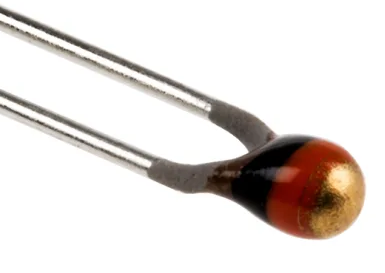
\includegraphics[width=\textwidth]{images/ctn.png}
        \caption{Thermistance CTN}
        \label{fig:sousfig2}
    \end{subfigure}
    \label{fig:figureprincipale}
\end{figure}


La thermistance de type CTN utilisée est un composant dont la résistance électrique vaut $R_0 = 10.0 \operatorname{k\Omega}$ quand la température vaut $T_0 = 25.0 \,^\circ C$ et dont la résistance électrique $R_{TH}$ varie en fonction de la température $T$ (en K) selon la loi de Steinhart–Hart (avec $B = 4300\operatorname{K}$) :
$$ \frac{1}{T} = \frac{1}{T_0} + \frac{1}{B} \ln \left( \frac{R_{TH}}{R_0} \right)$$

\Real Calculer la valeur de la thermistance $R_{TH}$ pour la température ambiante actuelle et en déduire la valeur théorique de la tension de sortie du pont de Wheatstone. \textit{Un thermomètre est à disposition dans la salle.}

\Real Prendre 3 résistances $R = 10 \operatorname{k\Omega}$ (pour $R_1$, $R_2$ et $P$) et mesurer leurs valeurs exactes. Vérifier la pertinence des valeurs trouvées par rapport à la couleur des anneaux présents sur la résistance. En déduire la valeur de tension attendue en sortie du pont de Wheatstone en prenant en compte les valeurs exactes de ces résistances.

\Real Câbler le montage du pont de Wheatstone et vérifier par la mesure la tension en sortie de celui-ci. 

\newpage

On se propose de remplacer la résistance $P$ par un \textbf{potentiomètre multitour} de valeur $P = 47\operatorname{k\Omega}$, dont la résistance varie entre les broches 1 et 2 du composant de $0$ à $47 \operatorname{k\Omega}$ selon la position du curseur.


\begin{figure}[h!]
    \centering
    \begin{subfigure}[b]{0.7\textwidth}
        \centering

\begin{circuitikz}[scale=0.8]
\draw 
  (0,0) to[R=$P$] (3,0);

  \draw[thick] (4,-0.3) -- (4.9,-0.3);     % Trait du bas
  \draw[thick] (4,0) -- (4.9,0); % Trait du milieu
  \draw[thick] (4,0.3) -- (4.9,0.3); % Trait du haut	
			
\draw (6,0) to[pR=$P$, mirror, name=R3] coordinate(tapR) (10,0);
        \draw (R3.wiper) --  ++ (1.25,0)  |- (tapR) to[short, -*] (tapR);
\end{circuitikz}     
        
        
        \caption{Câblage du potentiomètre}
        \label{fig:sousfig1}
    \end{subfigure}
    \hfill
    \begin{subfigure}[b]{0.2\textwidth}
        \centering
        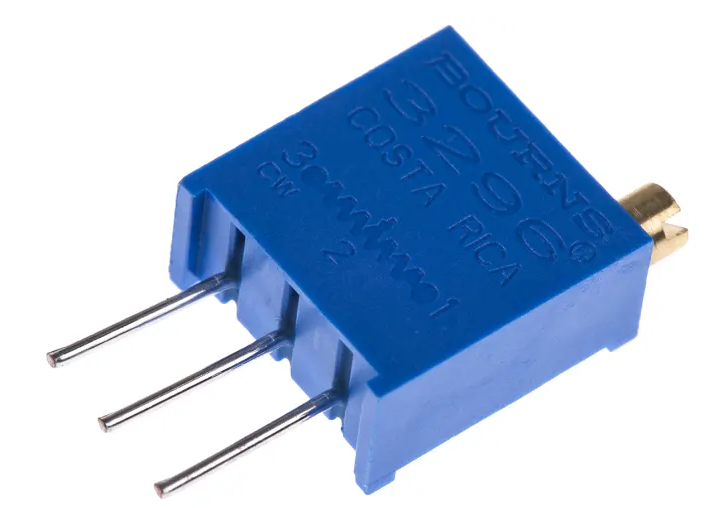
\includegraphics[width=0.6\textwidth]{images/trim.png}
        \caption{Potentiomètre}
        \label{fig:sousfig2}
    \end{subfigure}
    \label{fig:figureprincipale}
\end{figure}

\Real Que va permettre l'ajout de ce potentiomètre ? Modifier votre montage et régler la tension de sortie à une tension nulle pour la température ambiante actuelle.


%%%%%%%%%%%%%%%%%%%%%%%%%%%%%%%%%%
\subsection*{A2 - Alimentation symétrique}
\parpic[r]{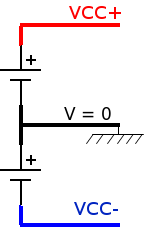
\includegraphics{images/Alim_cablageVCC.png}}

\Real Réaliser une alimentation symétrique de +$V_{CC}$ / -$V_{CC}$ (avec $V_{CC} = 5~V$) à l'aide de l'alimentation continue composée de deux blocs indépendants (voir document annexe \textit{Description du matériel} et figure ci-contre).

\Real Proposer et mettre en oeuvre une méthode de validation de ces deux tensions (successivement).
	

%%%%%%%%%%%%%%%%%%%%%%%%%%%%%%%%%%
\subsection*{A3 - Amplification du signal}

Le composant AD620 est un \textbf{amplificateur d'instrumentation} dont le schéma de câblage est représenté ci-dessous:
	
	\begin{center}
		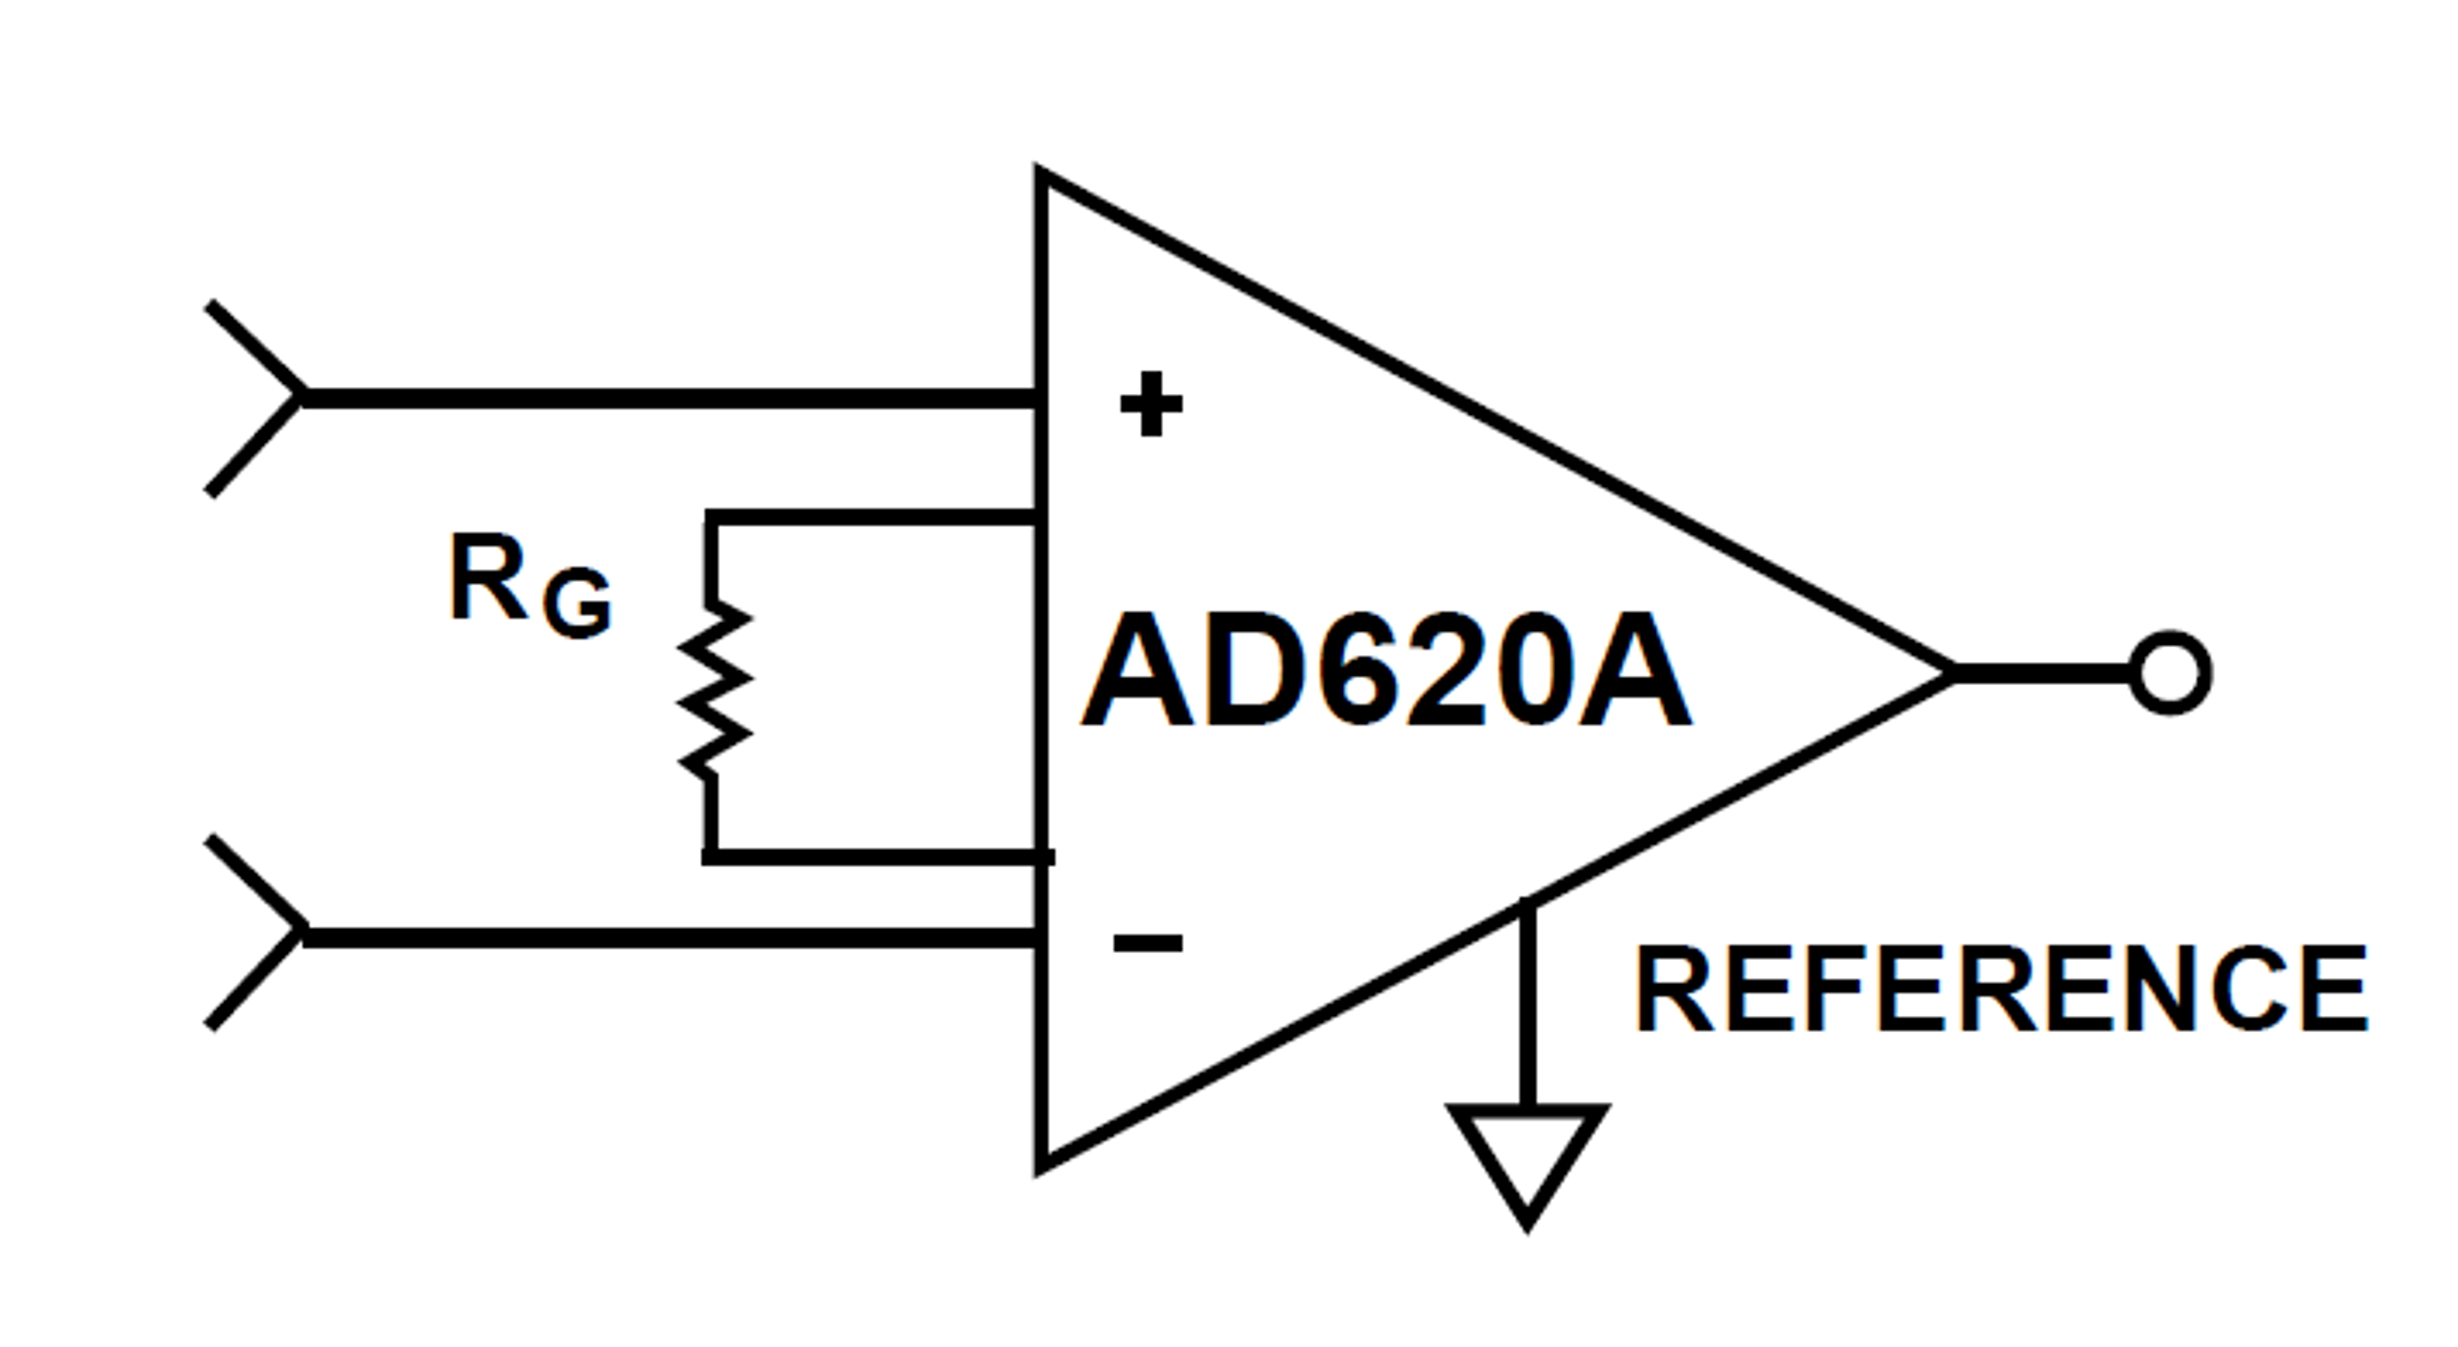
\includegraphics[width=4.5cm]{images/AD620.png}
		\hspace{1 cm}
		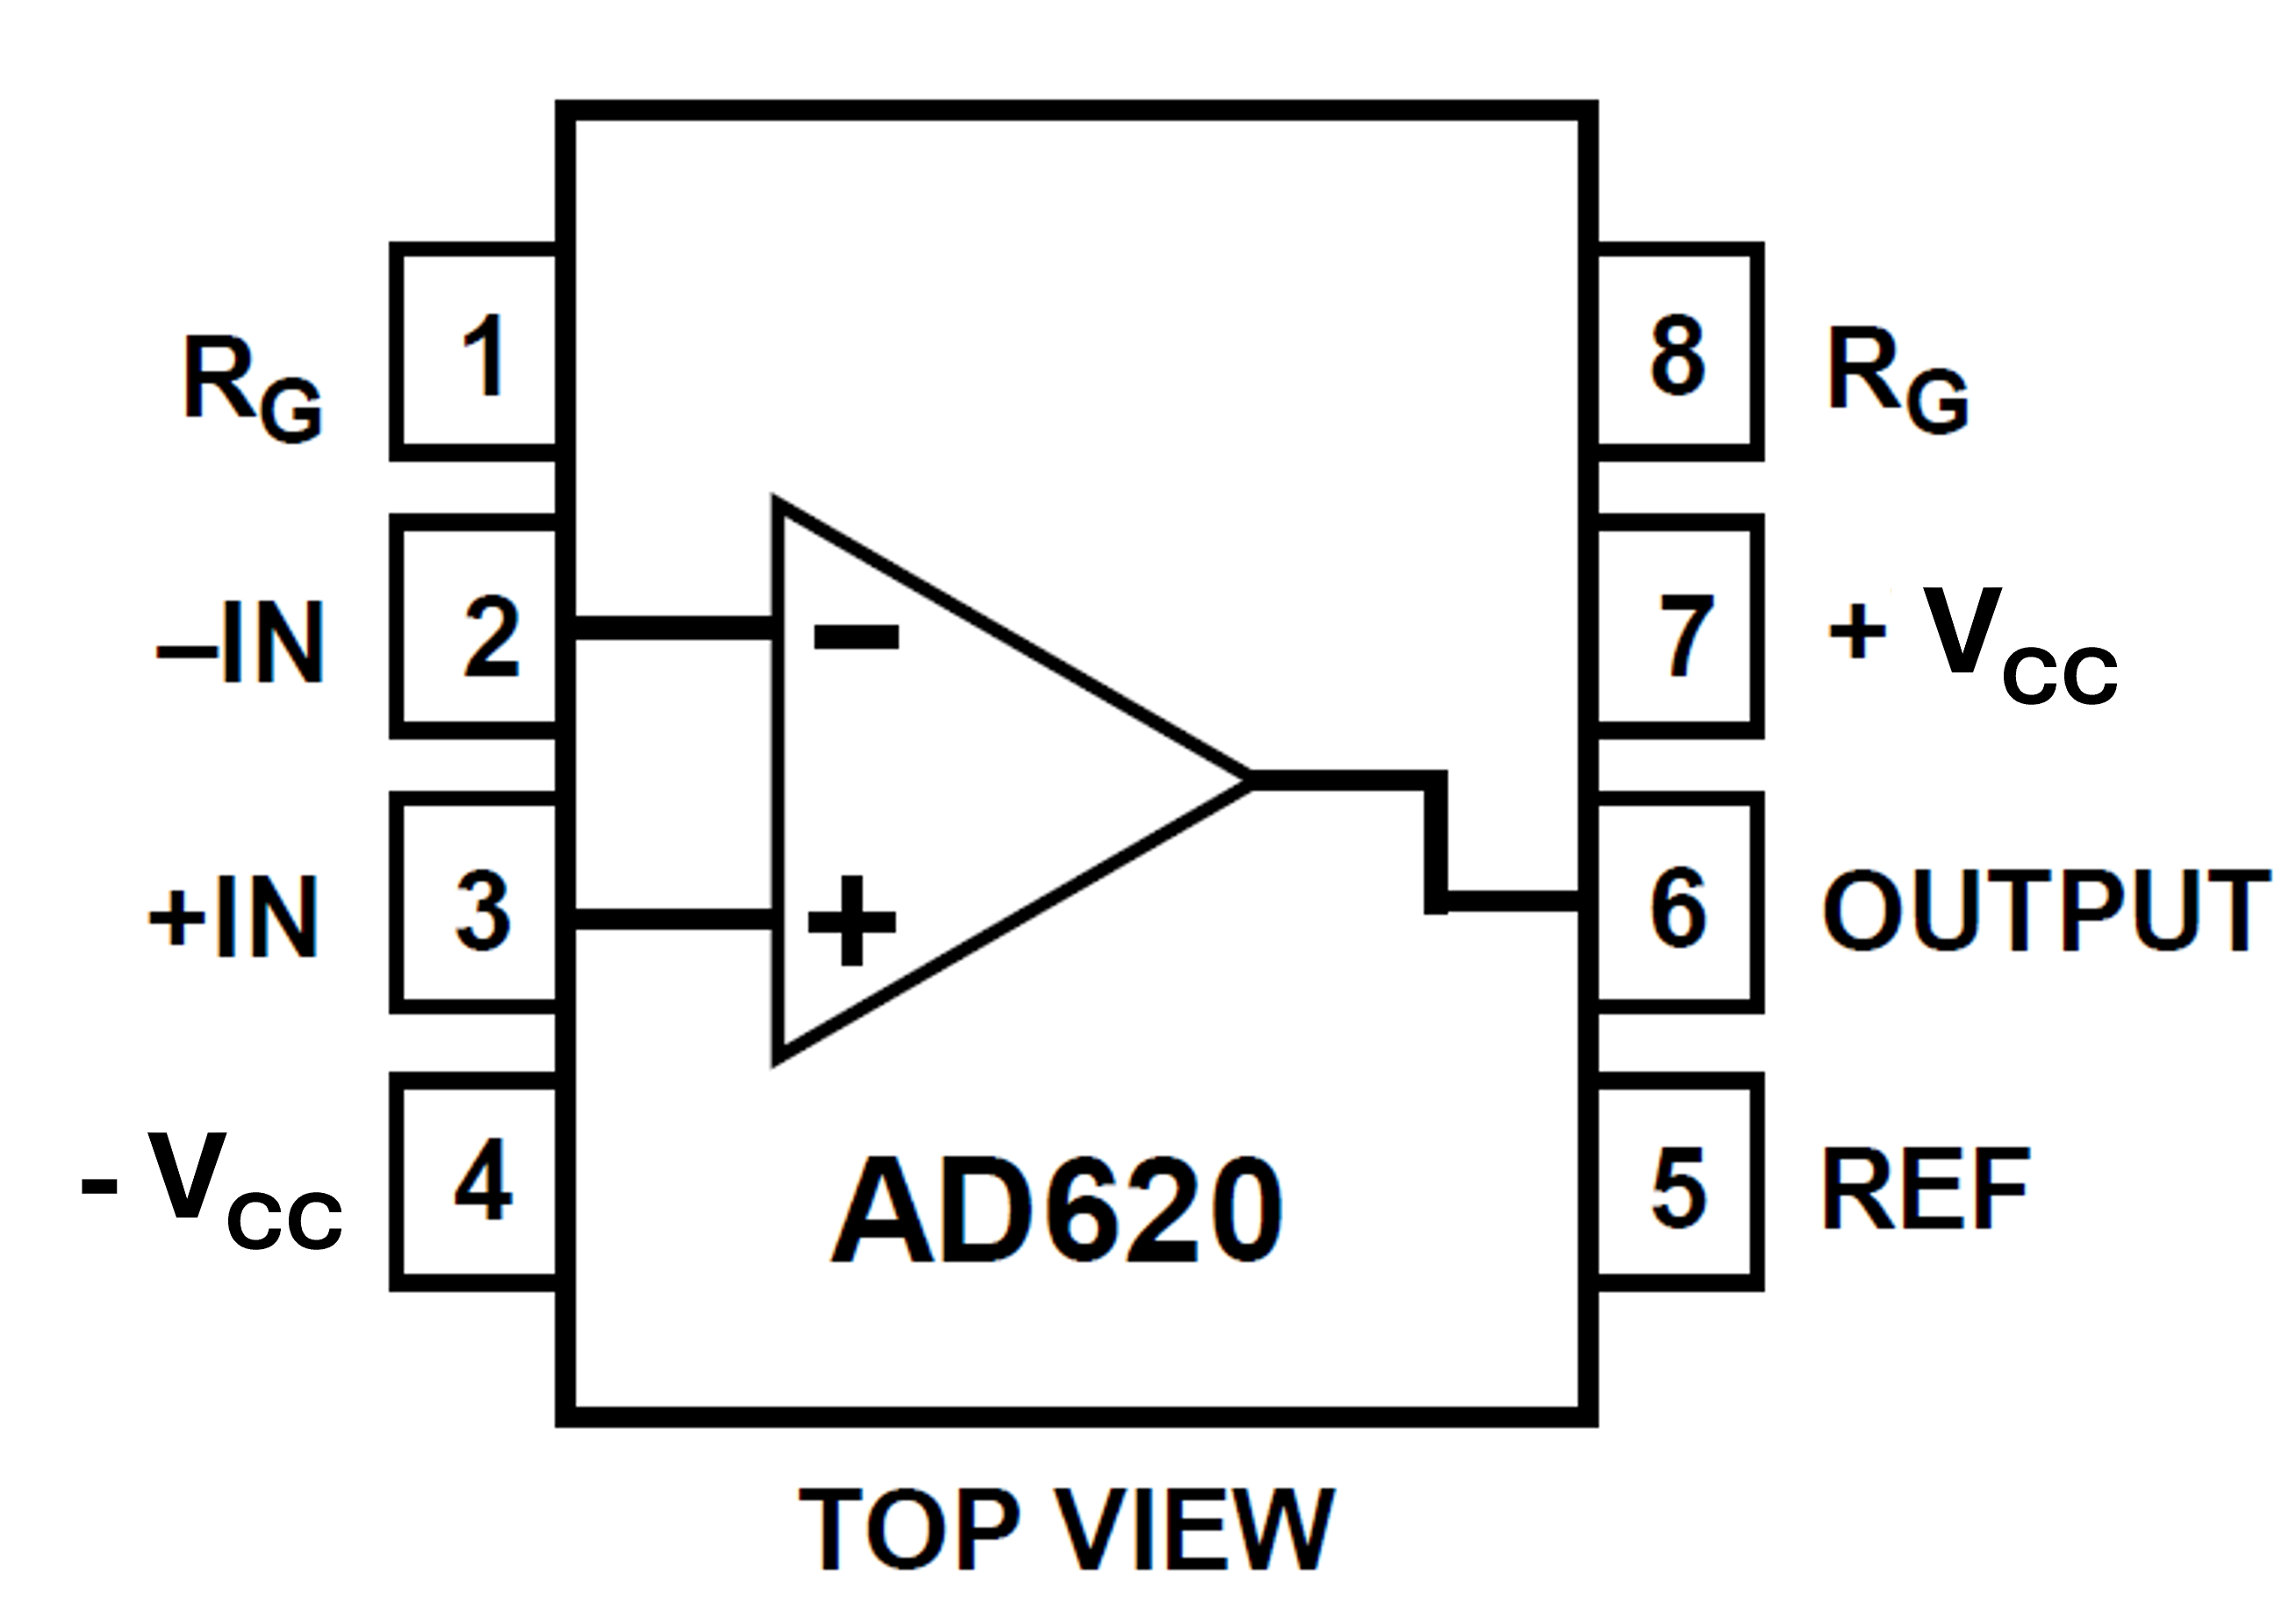
\includegraphics[width=4.5cm]{images/AD620SOIC.png}
	\end{center}
	
Le gain $G = \frac{V_s}{V_+ - V_-}$ entre sa sortie $V_s$ et ses entrées $V_+$ et $V_-$ dépend de la valeur de la résistance externe $R_g$ choisie selon l'équation:
$$G = \frac{49,4 \,k\Omega}{R_g}+1$$.

\Real Déterminer la valeur de $R_g$ permettant d'obtenir une plage de tension comprise entre $-5 \,V$ et $+5 \,V$ lorsque la température ambiante varie entre $15,0 \,^\circ C$ et $40,0 \,^\circ C$.

\Real Câbler le montage de l'AD620 en cascade avec le pont de Wheatstone avec une valeur approximative de $R_g$ déterminé précédemment et vérifier le bon fonctionnement de l'ensemble du circuit.


\newpage

\section{PARTIE B - Commande en puissance \textsc{\normalsize(Durée conseillée : 90 min)} }

On se propose maintenant d'étudier le \textbf{boitier annexe} fourni qui intègre un \textbf{composant numérique} ainsi qu'un composant de puissance.

\begin{center}
	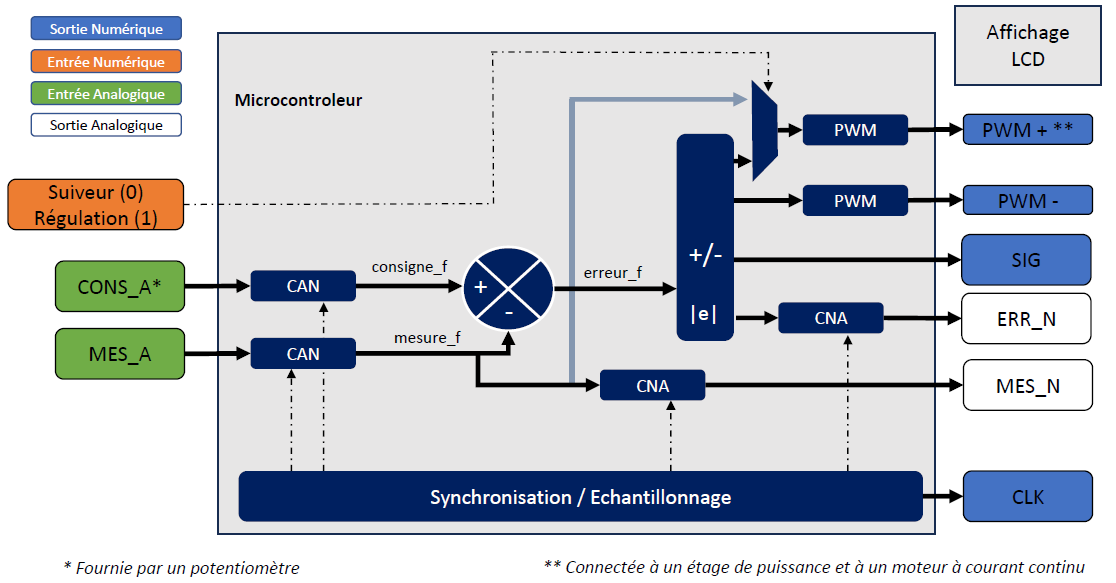
\includegraphics[width=\textwidth]{images/maquette_regul.png}
\end{center}

%%%%%%%%%%%%%%%%%%%%%%%%%%%%%%%%%%%%%%%%%%%%%
\noindent \rule{\linewidth}{1pt}

\textbf{\large \textsc{Attention : le boitier doit être alimenté entre 0 et 5V. Aucune tension négative n'est tolérée sur l'alimentation !}}

\noindent \rule{\linewidth}{1pt}

L'entrée \textbf{\textsc{MES\_A}} accepte des tensions pouvant aller entre $-1.5\operatorname{V}$ et $1.5\operatorname{V}$.

\subsection*{Mode de fonctionnement}

Le mode de fonctionnement peut être choisi à l'aide d'un interrupteur sur le boitier :

\begin{description}
	\item[Position 0] "\textit{Suiveur}" numérique - la sortie \textbf{\textsc{PWM+}} est directement contrôlée par le signal appliqué sur l'entrée \textit{CONSIGNE} (potentiomètre).
	\item[Position 1] "\textit{Régulation}" - la sortie \textbf{\textsc{PWM+}} est pitotée par le signal d'erreur entre la consigne et la mesure.
\end{description}


\subsection*{B1 - Etude de la sortie de mesure numérique du boitier}

\Real Placer le boitier en position "\textit{Suiveur}".

\Real Appliquer un signal sinusoïdal de $1\operatorname{V}$ d'amplitude crête à crête, de valeur moyenne nulle et de fréquence $1\operatorname{kHz}$ sur l'entrée \textbf{\textsc{MES\_A}}. 

\textbf{Vérifier au préalable votre signal à l'oscilloscope, pour ne pas endommager le boitier annexe.}

\Real Observer la sortie \textbf{\textsc{MES\_N}} du boitier. 

\Real Analyser le signal obtenu et indiquer les valeurs numériques des grandeurs caractérisant le fonctionnement de ce type de système. Faire une étude fréquentielle (basée sur la FFT) en testant plusieurs fréquences pour le signal d'entrée. 

\Real Que pouvez-vous conclure sur les limites d'utilisation de ce "Suiveur" ?


\subsection*{B2 - Commande numérique}


\Real Observer la sortie \textbf{\textsc{PWM+}} du boitier en fonction de la valeur de la consigne (potentiomètre). Expliquer en détail le lien entre l'entrée et la sortie du boitier. \textit{La sortie \textbf{\textsc{ERR\_N}} - dans le mode Suiveur uniquement - est une image de la tension en sortie du potentiomètre de consigne.}


\subsection*{B3 - Etage de puissance et moteur}

On décide de placer un moteur à courant continu (simulant un système de ventilation) qui sera piloté par la sortie \textbf{\textsc{PWM+}}. On insère un étage de puissance (déjà inclus sur la maquette) composé d'un transistor entre cette sortie et les broches du moteur.

\Real Expliquer le rôle d'un étage de puissance à cet endroit du montage.

\Real En faisant varier la consigne (potentiomètre), expliquer le principe de pilotage du moteur à courant continu.

\textbf{Le moteur doit être alimenté en  $6\operatorname{V}$ entre la masse (GND) et l'entrée de puissance  \textit{V\_MOT}.}

\textit{On rappelle que le moteur à courant continu peut-être considéré comme un convertisseur électrique-mécanique avec un comportement de type passe-bas de faible fréquence de coupure.}


\subsection*{B4 - Régulation}


\Real Placer le boitier en position "\textit{Régulation}".

\Real Appliquer un signal sinusoïdal de $1\operatorname{V}$ d'amplitude crête à crête, de valeur moyenne nulle et de fréquence inférieure à $1\operatorname{Hz}$ sur l'entrée \textbf{\textsc{MES\_A}}.

\Real Visualiser à l'oscilloscope les signaux \textbf{\textsc{PWM+}}, \textbf{\textsc{SIG}} et \textbf{\textsc{ERR\_N}}. Expliquer le rôle de chacun de ces signaux.

\Real Relever les informations pertinentes pour expliquer l'intérêt de cascader l'ensemble de ces montages pour obtenir la régulation de température souhaitée. \textit{L'amplitude du signal d'entrée (\textit{MES\_A}) peut être comprise entre $0$ et $2\operatorname{V}$.}

\Real Indiquer les limites de fonctionnement de ce système de régulation de température.

\Real Mettre en cascade les différents éléments et visualiser les signaux pertinents.




%%%%%%%%%%%%%%%%%%%%%%%%%%%%%%%%%%%%%%%%%%%%%%%%%%%%%%%%%%%%%%%%%%%%%%%%%%%%%%%%%%%%%
\end{document}
